\chapter{Background}

\section{Overview of Android OS}

The Android architecture
is structured in a series of layers (see \ref{fig:androidsystem}) offering different components and functionalities at different levels of abstraction, from hardware to system applications.
The bottom layer is composed by the Linux Kernel. This is the core system of Android, on top
of which all the components and layers are deployed. It also manages some of the most important security related policies. The next layer, in ascending order, is the \ac{hal}, in charge of allowing access to the hardware from components in upper layers.
It contains independent modules for each hardware component.

\begin{figure}[htbp]
  \centering
  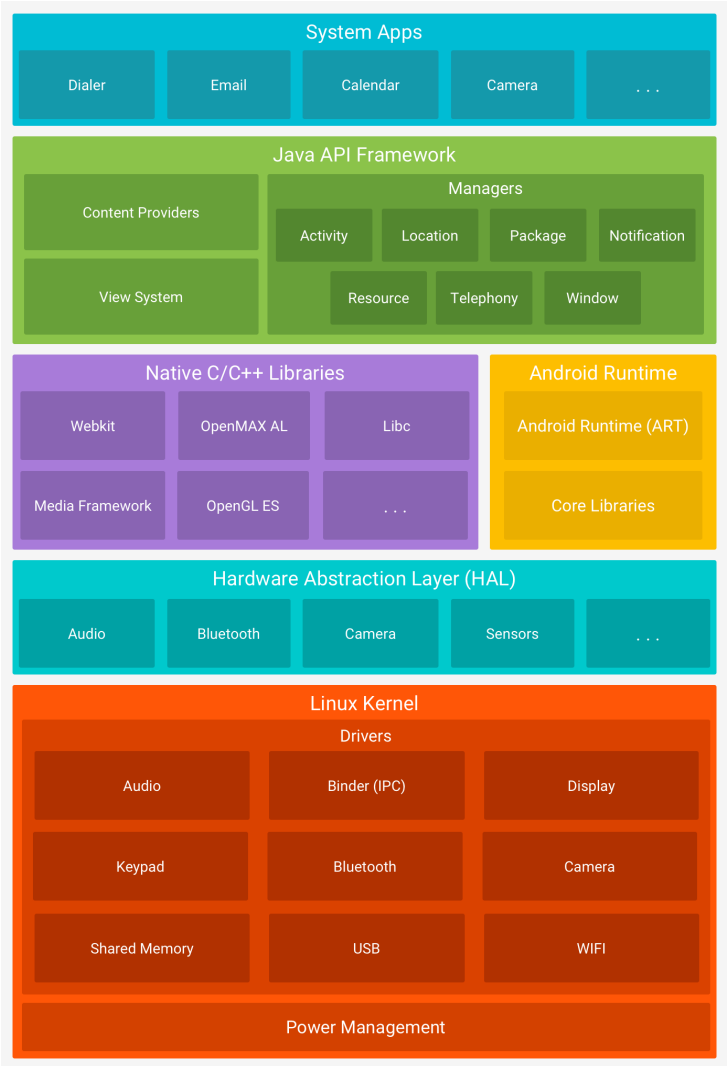
\includegraphics[scale=0.65]{./Figure/androidsystem.png}
  \caption{Android operating system architecture}
  \label{fig:androidsystem}
\end{figure}

Two layers are placed above. The first one, the Native C/C++ Libraries, used by developers who build their applications in any of these programming languages or also employed by
the Java \ac{api}. The second one is the \ac{art}, which has replaced Dalvik.
This environment allows running multiple virtual machines where applications developed in Java
execute in isolation.

On top of the two previously described parallel layers, it is possible to find the Java \ac{api}
framework. Through this \ac{api}, it is possible to access all functionalities offered by the Android
Operating system. The main objective of this layer is to facilitate the process of developing new
applications or reusing code in a rich environment designed to help the developer. Finally, the
top layer contains a set of system applications. They provide basic functionalities to the user,
such as internet browser, phone, email or calendar, but they can be replaced by other applications
installed by the user.

In Android, applications are distributed in files with extension .apk, which stands for \ac{apk}. These compressed files in zip format contain the necessary code, data, and
resources required to execute the application. 

\section{APK file structure}

\begin{figure}[htbp]
  \centering
  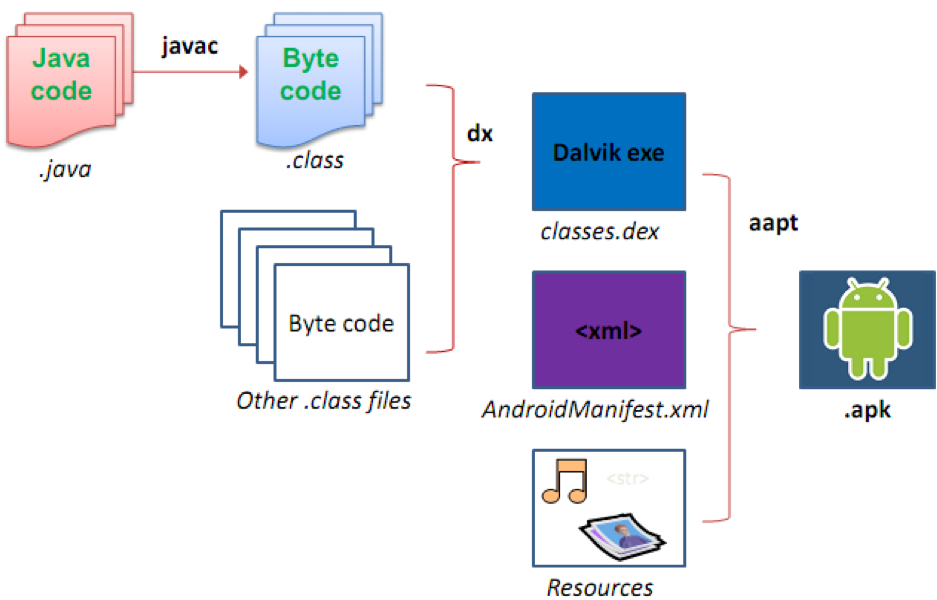
\includegraphics[scale=0.6]{./Figure/apkfile.png}
  \caption{Overview of the different files and folders obtained after unzipping an \ac{apk}}
  \label{fig:apk}
\end{figure}

Figure\ref{fig:apk} presents an overview of the different files and folders obtained after unzipping an \ac{apk}. However, since some of these files contain encrypted information, it is required to use specific tools such as AndroGuard \cite{androguard} or Apktool\cite{apktool} to extract the human readable
version of each file. The files contained in the different folders provide varied information which
can be used to categorize the behavior of the sample. For instance, /META-INF/ includes certificates, developer information or information to run the jar file. /assets/, resources.arsc and
/res/ are related to different mechanisms to import resources. The /lib/ folder stores compiled
libraries. Finally, two files provide the most relevant features when facing a malware analysis
task and which are shown in Figure\ref{fig:androidsystem}. classes.dex defines the code of the application in the
form of Dalvik bytecode. From here, a list of API calls, system commands or receivers defined
can be retrieved. The second important file is the AndroidManifest.xml, which declares a list of
permissions, the package name or a relation of intent filters.

\section{Android Malware}

Android malware applications primarily consist of
Trojans. A typical Android Trojans might trick the
user by using icons or user interfaces that mimic a
benign application. Android Trojans often display a
service level agreement during installation which
obtains permissions to access a user’s personal
information, such as the phone number. The Trojan
can then, for example, send SMS to premium rate
numbers in the background.
Android Trojans are also often used as spyware.
Such malicious applications can gain access to a
user’s private information and send it to a private
server. The main purpose of such spyware is to steal
information such as phone location, bank or credit
card details, passwords, text messages, contacts,
online browsing activity, and so on. A more
sophisticated implementation might also include
botnet capabilities.


\section{Analysis techniques for applications}
\subsection{Static Analysis}
In the static analysis, the analysis of the applications is done and the features are extracted without executing the application on an emulator or device. In comparison to other analysis techniques for android malware detection, static analysis consumes fewer resources and time as it does not involves execution of the application. The major disadvantage of this analysis is code obfuscation because of which detecting the malicious behavior of the application becomes difficult as pattern matching is not possible. This analysis can detect runtime errors, logical inconsistencies, and possible security violations.

Also static analysis includes the use of
reverse engineering techniques in order to access the set of instructions that define the application
operation. Furthermore, and focused on the Android platform, a large variety of characteristics
can be revealed using this kind of analysis. Information gathered from the Android Manifest or
from the resources are included into this category.

\subsection{Dynamic Analysis}

Dynamic analysis is the testing and evaluation of a program by executing data in real-time. The objective is to find errors in a
program while it is running, rather than by repeatedly examining the code offline. It is a detection technique which aims at
evaluating malware by executing the application and the main advantage of this technique is that determines the application
behavior during runtime and loads target data. The resource consumption in this analysis technique is more as compared to static
analysis. Dynamic behavioral detection method constructs operation environment by using a sandbox, virtual machine, and other
forms, and simulates the execution of the application to acquire the application’s behavior model.

\subsection{Hybrid Analysis}

Hybrid Analysis is a combination of static and dynamic analysis. It is a technology or method that can integrate run-time data
extracted from dynamic analysis into a static analysis algorithm to detect behavior or malicious functionality in the applications.
The hybrid analysis method involves combining static features obtained while analyzing the application and dynamic features and
information extracted while the application is executed. Though it could increase the accuracy of the detection rate, it makes the
system cumbersome and the analysis process is time consuming. 

\section{State-of-the-art machine learning algorithms for Android malware detection}

This section summarizes the most used machine learning classification algorithms in the literature
related to Android malware detection and family classification.

\subsection{Decision Trees}

Decision trees are one of the former machine learning methods for regression and classification.
They provide a useful mechanism based on a set of splitting rules. These models make
a prediction based on the most common class in the region of the example. Typically, decision
trees are generated through consecutive binary splitting while an error function is minimized. One
of the strengths of these models lies in that they allow an easy interpretation and visualization.
In contrast, they have several drawbacks, such as classification problems when presenting data
with small changes. An example of decision tree algorithm is ID3, which makes divisions
trying to maximize the information gain.

\subsection{Random Forest}

Decision trees are one of the simplest learning
techniques. However, a decision tree tends to overfit
the training data, since it is a literal interpretation of
the data, and provides no generalization of the training set. To partially alleviate this problem,
multiple decision trees can be used, where each is
trained on a subset of the training data. A random
forest takes this idea one step further by also training
on subsets of the classifiers \cite{breiman}.
Although much of the inherent simplicity of decision
trees is lost in this process, random forests have
proved to be a very strong machine learning
technique over a wide variety of applications. 

\subsection{K-nearest neighbors}

The K-nearest neighbors is a non-parametric classifier, meaning that this model grows in parallel
to the size of the training data \cite{rob14}. Basically, it uses a distance metric to provide a prediction
based on the majority class among the K nearest point to the example. While these models have
proved to be powerful in varied problems, they are not indicated for high-dimensional spaces.

\subsection{Support Vector Machine}

This is a powerful algorithm used for both classification and regression problems. It is based on
representing each example in a n-dimensional space, where a hyperplane is created pursuing the
best separation between classes \cite{svm}. For building this hyperplane, a portion of the training
data called support vectors is employed. These models have been widely used in the literature
for building malware detection tools.

\subsection{Logistic Regression}

Logistic regression is the appropriate regression analysis to conduct when the dependent variable is dichotomous (binary). \cite{logic} Like all regression analyses, the logistic regression is a predictive analysis.  Logistic regression is used to describe data and to explain the relationship between one dependent binary variable and one or more nominal, ordinal,interval or ratio-level independent variables.

\subsection{Gradient boosting}
Gradient boosting is a machine learning technique for regression and classification problems, which produces a prediction model in the form of an ensemble of weak prediction models, typically decision trees. It builds the model in a stage-wise fashion like other boosting methods do, and it generalizes them by allowing optimization of an arbitrary differentiable loss function.

Nowadays we have some state-of-the-art algorithms implementing Gradient boosting.
Below, we introduce the top 3 of the most used algorithm implementing Gradient boosting.

\subsubsection{XGBoost}

XGBoost is an algorithm that has recently been dominating applied machine learning and Kaggle competitions for structured or tabular data.

XGBoost is an implementation of gradient boosted decision trees designed for speed and performance created by Tianqi Chen, now with contributions from many developers. \cite{xgboost}

\subsubsection{LightGBM}

LightGBM is a gradient boosting framework that uses tree based learning algorithms. It is designed to be distributed and efficient with the following advantages: Faster training speed and higher efficiency,
Lower memory usage,
Better accuracy,
Support of parallel and GPU learning,
Capable of handling large-scale data. \cite{lgbm}

\subsubsection{Catboost}

CatBoost is an algorithm for gradient boosting on decision trees. It is developed by Yandex researchers and engineers, and is used for search, recommendation systems, personal assistant, self-driving cars, weather prediction and many other tasks at Yandex and in other companies, including CERN, Cloudflare, Careem taxi. It is in open-source and can be used by anyone. \cite{cat}

\subsection{Artificial Neural Networks}

Artificial neural networks are algorithms that can be used to perform nonlinear statistical modeling and provide a new alternative to logistic regression, the most commonly used method for developing predictive models for dichotomous outcomes in medicine. Neural networks offer a number of advantages, including requiring less formal statistical training, ability to implicitly detect complex nonlinear relationships between dependent and independent variables, ability to detect all possible interactions between predictor variables, and the availability of multiple training algorithms. \cite{neuralnets}